In this chapter we will present in detail and discuss the Random
Linear Economy model \cite{DeMartinoMarsili04} developed by Andrea De
Martino, Matteo Marsili and Isaac Pérez Castillo which will be the
basis for some of the applications discussed in the second part of
this thesis.

There are some reasons why we chose to work with this model in
particular: first, it presents a General Equilibrium Model which has
few ingredients but displays a rich behavior, including phase
transitions which depend on the number of firms in the
market. Secondly, it is analytically solvable using Statistical
Mechanics techniques, such as using the replica method to calculate the
partition function. Therefore, it was ideal for trying new venues of
exploration without the difficulty imposed in trying to prove general
results. 

\section{The Model Ingredients}

A model economy is composed by two types of actors: consumers and firms. We assume $N$
firms and one single representative consumer with utility function
$U(x)$ and initial endowment $x_0$. As we mentioned on Chapter \ref{cha:GET}, this is a common approximation
when doing equilibria calculations in Economics due to its simplicity:
if we have $J$ consumers with independent utility functions $U_j$ (i.e.,
$U_j$ never depends on $x_k$, $k\neq j$) and initial endowments
$\omega_j$, then either we do not allow wealth transfers of $\omega_j$
and the optimization problem becomes very complicated, or we allow the
central authority to carry out wealth transfers prior to allocation,
and then the the demands generated by the consumers in this scenario
is equivalent to that of a single representative consumer with utility
function $U_R = \sum_{j=1}^J U_j$ and wealth
$\omega_R = \sum_{j=1}^J \omega_j$.

The representative consumer assumption receives considerable criticism
\cite{Kirman92}, chiefly because disregarding interaction among agents
(via the utility of one depending on the decisions of the others)
washes out the possibility of interactions and the wide range of
important and interesting phenomena that in the statistical physics
community we know to be generated precisely by these interactions
\cite{Bouchaud13}, whereas the representative agent is a mean field
approximation for consumers.

The representative consumer is used in this model precisely
because it generates an energy function which is convex and therefore has a
well defined, unique minimum. Besides, the resulting partition function can
be calculated analytically in the zero temperature limit. The interactions are at the supply side, which we will describe next, and are enough to generate rich behavior even with the representative consumer approximation.

The consumer and $N$ firms will trade $M$ goods, with a density parameter given by $n = N/M$. As with General Equilibrium settings, we assume the consumer has an initial wealth
$x_0 = (x_0^1, \ldots, x_0^M)$, $x_0^\mu \geq 0$, and wishes to
improve its welfare in the market by using his endowment $x_0$ to
purchase a consumption bundle $x$ according to a separable utility
function $U(x) = \sum_{\mu=1}^M u(x^\mu)$. His initial endowment,
however, is random, with each $x_0^\mu$ drawn independently
from an exponential distribution with unitary scale, i.e.,

\begin{equation}
  \label{eq:rle_1}
  P(x_0^\mu) = e^{-x_0^\mu}
\end{equation}

This particular form of distribution for the initial endowments is chosen so the consumer has a large imbalance of initial goods for which he needs the market to improve on. As before, the aim of the consumer in this economy is to solve the utility
maximization problem

\begin{equation}
  \label{eq:rle_3}
  x^\ast = \argmax_{x} U(x) \text{ s. t. } p\cdot x \leq p\cdot x_0
\end{equation}

We will treat the
particular case of the consumer's utility being a separable function $u(x_\mu) = \log x_\mu$, although any concave function would exhibit qualitatively similar behavior. The logarithm is a common choice for the consumer's utility function because it satisfies some of the  properties desired for the consumer behavior in Economics. The often called the Inada conditions are: first, the consumer is \textbf{loss averse}, which means that he will
always prefer a guaranteed amount $a$ of any good to a lottery in
which he can win $a + \delta$ with probability 0.5 and $a - \delta$
with probability 0.5, for any $\delta > 0$. He is loss averse because
the disutility losing $\delta$ is larger than the utility of gaining
$\delta$. We don't have any stochastic payoff such as lotteries in the model, but the principle
holds for two goods: if he has $\bar{x} - \delta$ of good $\mu$ and
$\bar{x} + \delta$ of good $\nu$, he will try to find a company that
trades this excess of good $\nu$ so he can average both goods and may even do so at a loss (i.e., he ends up with
$\bar{x} - \varepsilon$ for both goods, for some
$\varepsilon < \delta$). Furthermore, with separable utility as chosen,
there are no complementary or substitute goods, i.e., goods for which
the consumer prefers to have more (or less) of one if he has
another. Finally, because $u(0) = -\infty$, the consumer will always
try to obtain a little bit of every good, even if at a great cost,
because nothing is worse than having none of a particular good.

Each firm, on the other hand, has an $M$-dimensional random
technology $\xi_i = (\xi_i^1, \ldots, \xi_i^M)$, where $\xi_i^\mu<0$
represents an input and $\xi_i^\mu>0$ represents an output. The
production set of each firm is the space of all vectors which are
proportional to $\xi_i$, that is, $\Xi_i = s \xi_i$, $s \geq 0$. Each firm $i$ only has one technology and its only decision
is the scale $s_i$ at which it operates this technology. Once chosen
the scale $s_i$, a company will consume $s_i \xi_i^-$ goods and
produce $s_i \xi_i^+$ goods, where $\xi_i^{\pm}$ are the positive and
negative entries of the $\xi_i$ vector.

The elements $\xi_i^\mu$ are initially independently drawn from a normal
distribution with zero mean and $\Delta/M$ variance, where $\Delta >
0$ but are then normalized so that the
sum over all the goods for a company is fixed at a negative value and
all technologies are a little inefficient. We must have then:

\begin{align}
  \label{eq:rle_2}
  P(\xi_i^\mu) & = \mathcal{N}(\xi_i^\mu | 0, \Delta M^{-1}) \\ \sum_{\mu=1}^M
  \xi_i^\mu & = -\epsilon
\end{align}


We normalize the technologies to be inefficient so that we don't have
a combination of firms producing infinite goods, i.e., firm $i$
and $j$ can produce infinite amounts of certain goods by each feeding
its output to be used as the other's input. This would make the economy violate the second law of Thermodynamics, which is surely an undesirable property for any practical model of a closed economy.

The objective of each company in the market is the same as before:
each firm $i$ tries independently to choose it's production scale
$s_i$ as to maximize it's profits:

\begin{equation}
  \label{eq:rle_6}
  s_i^\ast = \argmax_{s_i > 0} p\cdot (s_i \xi_i)
\end{equation}

Other underlying assumptions of General Equilibrium Theory are valid
here: we assume a complete market, where each agent knows the offer
and demand of all other agents, there is no transaction costs and a
good is uniquely defined. Also, agents are price-takers, which means
that they have no power over the prices and must accept them as given.

We also treat the economy as closed and therefore it must satisfy the market
clearing condition. Because we have just one consumption bundle, then
the $N$ dimensional production scale vector $s$ has to be such that

\begin{equation}
x = x_0 + \sum_{i=1}^N s_i \xi_i
\label{eq:market_clearing}
\end{equation}
ie, all the inputs the firms use have to come from the consumer's
initial endowment. If we sum over all the goods we have a strict condition on the final conversions from $x_0$ to $x$:

\begin{equation}
\label{eq:mc_eff}
  \sum_{\mu = 1}^M x_\mu - x_0^\mu = -\epsilon \sum_{i=1}^N s_i
\end{equation}

Because market clearing hold and agents are price takers, we can also
derive the strong restriction on profits discussed before. If we
multiply both sides of the equation \eqref{eq:market_clearing} by $p$,
we get

\begin{equation}
  \label{eq:market_clearing_p}
  p\cdot (x - x_0) = \sum_i s_i p \cdot \xi_i,
\end{equation}

The left side of the above equation has to be less or equal
to zero as a consequence of the budget condition. But the right hand side has
to be always greater or equal to zero, because this term represents
the sum of the individual firms' profits and if a firm is losing money
they can always choose to set $s_i = 0$ and leave the
market. Therefore, we must have that both sides are equal to zero, and
the consequence is that the agent completely spends all his available
budget (i.e., $p\cdot x = p \cdot x_0$, he has not ``leftover'' cash
after choosing $x$, this is Walras's law for this model) and that the firms either have zero profit
($p\cdot \xi_i = 0$) or leave the market ($s_i = 0$).

One of the important implications of equation
\eqref{eq:market_clearing_p} for the Random Linear Economy model is
that we may have no more than $M$ firms active at any given
realization of equilibrium. If the right hand side of equation
\eqref{eq:market_clearing_p} has to be zero, then for every firm
either $s_i = 0$ or $p\cdot \xi_i = 0$. If $\phi$ is the fraction of
firms active in the market, that is

\begin{equation}
  \label{eq:phi_def}
  \phi = \frac{\sum_{i=1}^N \mathds{I}(s_i > 0)}{N},
\end{equation}
then all of them have $p\cdot \xi_i = 0$. Because the price is the
same for all of them, we have $\phi N$ equations of this type, and $M$
unknowns. For this system to have a non-trivial solution (ie,
$p_\mu > 0$ for all $\mu$), it must be that $\phi N \leq M$, which
implies that

\begin{equation}
  \label{eq:phi_max}
  \phi \leq \frac{1}{n}
\end{equation}

Having a single representative consumer (or
many consumers but with wealth transfers) has two important
consequences: first, the price vector is entirely determined by the
consumer's demand. This is a consequence of the first order condition for
the maximization problem. By taking the derivative of equation
\eqref{eq:rle_3} with the proper Lagrange multiplier we get

\begin{equation}
  \label{eq:rle_8}
  \frac{\del U(x)}{\del x_\mu} - \lambda p_\mu = 0 \Rightarrow p_\mu =
  \frac{1}{\lambda x_\mu}
\end{equation}

Furthermore, the market clearing condition binds the optimization
problem of the consumer and the firms. If we substitute equation
\eqref{eq:market_clearing} in the consumer's utility, we get:

\begin{equation}
  \label{eq:rle_7}
  s^\ast = \argmax_{s : s_i \geq 0} U(x_0 + \sum_{i=1}^N s_i \xi_i)
\end{equation}

We can easily check that the zero profit condition is preserved with
this solution. If $s_i$ is in $s^\ast$, the solution for the
consumer's maximization problem, then either $s_i = 0$ or $s_i >
0$. If $s_i = 0$, the condition is satisfied. Otherwise, if $s_i > 0$,
it means that the constraint $s_i \geq 0$ was not enforced and the
derivative at $s_i$ must be zero. We then have

\begin{equation}
  \label{eq:rle_9}
  0 = \frac{\del U}{\del s_i} = \frac{\del U}{\del x} \frac{\del
    x}{\del s_i} = p\cdot \xi_i
\end{equation}

Our problem is now considerably reduced: to find the equilibria in
this model economy all we have to do is to solve the maximization problem
in equation \eqref{eq:rle_7}.


\section{The Role of Statistical Mechanics} \label{sec:rle_statmech}

If we were to employ standard convex optimization techniques
to solve \eqref{eq:rle_7}, we would be able to find the solution for a
specific realization of $x_0$ and $\xi$ given a fixed $N$ and $M$. But
if we were to calculate quantities of interest such as consumer
utility, average good consumption, average good price, price deviation
among goods, number of active firms, etc, these would all be random
variables which depend on the realization of endowments and
technologies.

This is, of course, a well known setup in Statistical Mechanics. We
solve this by treating the case where the system size is very large,
so that these average quantities converge to a single value. This
isn't always the case, but holds for the so called
\emph{self-averaging} systems. In these systems, these average
quantities for large systems converge to an average over the
realizations for smaller systems.

The general approach to finding the equilibrium properties of a
physical system is is to calculate the partition function for a specific
realization of $\xi$, $x_0$:

\begin{equation}
  \label{eq:rle_10}
  Z(\beta | \xi, x_0) = \int dx e^{\beta U(x| x_0, \xi)},
\end{equation}
where $\beta$ is the inverse value of the temperature. From this, we
can calculate the average value of the utility function by taking the
derivative of $\log Z$:

\begin{equation}
  \label{eq:rle_12}
  \left \langle U \right \rangle (\beta | \xi, x_0) = \int_0^\infty dx
  \frac{e^{\beta U(x|\xi, x_0)}}{Z(\beta |\xi, x_0 } U(x|\xi, x_0) = \frac{\del}{\del \beta} \log Z(\beta | \xi, x_0)
\end{equation}

The maximum value for the utility $U(x)$ is equivalent to the average
value on the ground state\footnote{This is true because $U(x)$ is
  convex and therefore has only one maximum.}, ie:

\begin{equation}
  \label{eq:rle_13}
  \max_x U(x | \xi, x_0) = \lim_{\beta\to\infty} \langle U \rangle (\beta | \xi, x_0)
\end{equation}

However, we are still calculating the maximum as a function of the
samples $x_0$ and $\xi$. In order to get the average behavior, which
holds for a large system, we must average the utility over the
disorder. Writing it all explicitly, we finally get the solution
to equation \eqref{eq:rle_7}:

\begin{equation}
  \label{eq:rle_14}
  \max_x U(x) = \int d\xi dx_0 P(\xi) P(x_0)  \lim_{\beta\to\infty} \frac{\del}{\del \beta} \log \int dx e^{\beta U(x| x_0, \xi)}
\end{equation}
 
The analytical calculation of the expression above is considerably
involved and makes use of a method commonly known as \textbf{replica
  method} in the Statistical Physics community. We leave the lengthy calculation for Appendix \ref{app:rep}. The
solution of this calculation is given by

\begin{equation}
  \label{eq:rle_52}
  \lim_{N\to \infty} \frac{1}{N} \max_x \, U(x) = \max_\theta h(\Omega, \kappa,
  p, \sigma, \chi, \hat{\chi}),
\end{equation}
where $\theta = (\Omega, \kappa,
  \sigma, \chi, \hat{\chi})$ are order parameters that appear during
  the calculation and $h$ is given by:

\begin{align}
  \label{eq:h}
  h(\Omega, \kappa, p, \sigma, \chi, \hat{\chi})& = \left\langle
    \max_s \left[-\frac{\hat{\chi}}{2}s^2 + (t \sigma - \epsilon p)
                                                  s\right]
                                                  \right\rangle_t +
                                                  \nonumber\\ & +
  \frac{1}{2} \left(\Omega \hat{\chi} + \frac{\kappa p}{n}\right) -
  \frac{1}{2n\Delta} \chi \sigma^2 - \frac{1}{2n} \chi p^2 + \nonumber\\ &+
  \frac{1}{n} \left\langle \max_x \left[U(x) - \frac{(x - x_0 + \kappa +
      \sqrt{n\Delta\Omega}t)^2}{2\chi}\right] \right\rangle_{t,x_o},
\end{align}
where $t$ is a normal random variable with zero mean and unitary variance.

The zero temperature limit makes the terms involving $s$ and $x$ revert to the two original optimization problems of the firms and consumer, respectively. However, the extra terms couple those two maximization issues. Because we are in the thermodynamic limit where $M, N \to \infty$ with $n = N/M$ fixed, the maximization solution is a distribution over the $N$ productions scales and $M$ good quantities. The solution for $s^*$ is obtained by solving  $\frac{\del}{\del s}
\left[-\frac{\hat{\chi}}{2}s^2 + (t \sigma - \epsilon p) s\right] =
0$. Keeping in mind the constraint that $s\geq 0$, we have

\begin{equation}
  \label{eq:s_ast}
  s^*(t) =
  \begin{cases}
    \frac{(t\sigma - \epsilon p)}{\hat{\chi}}, & \text{if } t \geq \frac{\epsilon
      p}{\sigma} \\
    0, & \text{otherwise.}
  \end{cases}
\end{equation}

The probability distribution of $s$ has a mass on $s=0$, which has probability equal to the case where $t < \epsilon p / \sigma$, and a Gaussian probability distribution for $t \geq \epsilon p /
\sigma$. We can write it in closed form by integrating over $t$:

\begin{equation}
  \label{eq:rle_64}
  P(s) = \int_{-\infty}^\infty dt \frac{1}{2\pi}
  e^{-\frac{t^2}{2}} \delta (s - s^*)
\end{equation}

We use the identity that for the Dirac delta function $\delta(x - a) = |f'(a)|\delta(f(x))$ given any function $f(x)$ with a simple root in $a$. Choosing $f(s) = \frac{s\hat{\chi} + \epsilon p}{\sigma} - t$ we have

\begin{equation}
  \label{eq:rle_63}
  P(s) = (1 - \phi) \delta(s) + \Theta(s) \frac{\hat{\chi}}{\sqrt{2\pi}
    \sigma} e^{-\frac{(\hat{\chi}s + \epsilon p)^2}{2\sigma^2}},
\end{equation}
where $\phi = \frac{1}{2} \erfc\left(\frac{\epsilon p}{\sqrt{2} \sigma}\right)$ is the fraction of active firms ($s > 0$) in the economy.
    
In the same manner, the solution of the consumer's maximization problem on $x$ is given by the implicit equation obtained when solving $\frac{\del}{\del x} \left[U(x) - \frac{(x - x_0 + \kappa + \sqrt{n\Delta\Omega}t)^2}{2\chi}\right] = 0$:

  \begin{equation}
    \label{eq:x_ast}
    x^* = x : U'(x) = \frac{(x - x_0 + \kappa +
      \sqrt{n\Delta\Omega}t)}{\chi}
  \end{equation}

Using $f(x) = \frac{x - x_0 - \chi u'(x) + \kappa}{\sqrt{n \Delta \Omega}} + t$ for the same replacement as in \eqref{eq:rle_63} we have

\begin{equation}
  \label{eq:rle_66}
  P(x) = \frac{1 - \chi U''(x)}{\sqrt{2\pi n \Delta \Omega}} e^{-
    \frac{(x - x_0 - \chi U'(x) + \kappa)^2}{2n\Delta \Omega}}
\end{equation}

To find the maximum value of $h$ given the order parameters $\Omega, \kappa,
  \sigma, \chi, \hat{\chi}$, we must again take the derivative with respect to each of these parameters. These give us the so called \textbf{saddle point equations} which, despite being used to find the maximum of $h$ and therefore the expected value of the utility in a large system, also give us insights into the behavior of quantities of interest such as the good prices. The saddle point equations for equation \eqref{eq:h} are (see Appendix \ref{app:rep} for details):

\begin{align}
  p & = \left \langle U'(x^*) \right \rangle_{t,x_0} \label{eq:saddlep} \\
\Omega & = \left\langle (s^*)^2 \right\rangle_t \label{eq:saddleomega}\\
\sigma & = \sqrt{\Delta
    \left(\left \langle U'(x^*)^2 \right \rangle_{t,x_0} - \left
        \langle U'(x^*) \right \rangle_{t,x_0}^2 \right)} \label{eq:saddlesigma}\\
    \chi & = \frac{n\Delta}{\sigma} \left \langle t s^* \right
    \rangle_t \label{eq:saddlechi}\\
\hat{\chi} & = \sqrt{\frac{\Delta}{n\Omega}} \left \langle U'(x^*) t
\right \rangle_{t,x_0} \label{eq:saddlehatchi}\\
  \kappa & = p \chi + n\epsilon \left \langle s^* \right \rangle_t \label{eq:saddlekappa}
\end{align}

The equations above allow for some sanity checking: if we take the expected value of equation \eqref{eq:x_ast} with respect to $t$ and $x_0$ we have

\begin{equation}
  \langle \chi U'(x^\ast) \rangle_{t, x_0} = \langle x \rangle_{t, x_0} - \langle x_0 \rangle_{x_0} + \kappa + \langle \sqrt{n\Delta\Omega}t \rangle_{t, x_0}
\end{equation}

But the last term is the average of $t$ which is zero, and if we replace $\kappa = p \chi + n\epsilon \left \langle s^* \right \rangle_t$ and $\langle \chi U'(x^\ast) \rangle_{t, x_0}$ by $\chi p$ we have

\begin{equation}
    \langle x \rangle_{t, x_0} =  \langle x_0 \rangle_{x_0} - n\epsilon  \left \langle s^* \right \rangle_t,
\end{equation}
which is the thermodynamic limit version of equation \ref{eq:mc_eff}. 


\section{Regime change at $n=2$}

One of the most interesting aspects of this seemingly simple model it that it exhibits two very different economic behaviors, one when $n<2$ and the other when $n>2$: when $n < 2$, the economy is competitive, half of the firms in the market are active and operating but are not efficient enough that the consumer is completely satisfied, so new firms entering improve the consumer's utility and increase the economy's GDP. When $n > 2$, the market is saturated, monopolistic (most firms are inactive) and new firms entering have a negligible impact over the economy.

This behavior has a simple geometric explanation which can be shown without the results obtained above. If we write the initial endowments as $x_0 = \bar{x}_0 + \delta x_0$, such that $\bar{x}_0$ is the average (which has an expected value of one) and $\sum_\mu \delta x_0^\mu = 0$, then the consumer picks\footnote{Remember that market clearing couples the consumer's maximization problem with the firms'} $s$ as to minimize the dispersion vector $\delta x_0$ as much as possible. Therefore, firms that have $\xi_i \cdot \delta x_0 < 0$ will have a positive production scale, whereas firms that have $\xi_i \cdot \delta x_0 > 0$ will increase the dispersion of the initial goods, reducing the consumer's utility and therefore won't get used, having $s_i = 0$.

At the $\epsilon \to 0$ limit, each component $\xi_i^\mu$ is drawn from a normal distribution with zero mean, so the plane $\xi_i \delta x_0 = 0$ divides the set of firms in half, because each firm has equal probability of having its independent (when $\epsilon = 0$) technologies drawn in such a way that $\xi_i \cdot \delta x_0 < 0$, no matter what vector is $\delta x_0$ as long as it's not zero. This means at most $N/2$ are active at any given moment. However, we know from equation \eqref{eq:phi_max} that there can be at most $M$ firms active in the economy. Therefore, in the limit of $\epsilon \to 0$, we must have $\phi = 1/2$ up until $N/2 = M$, which implies a transition at $n = 2$.

\begin{figure}[!ht]
  \centering
  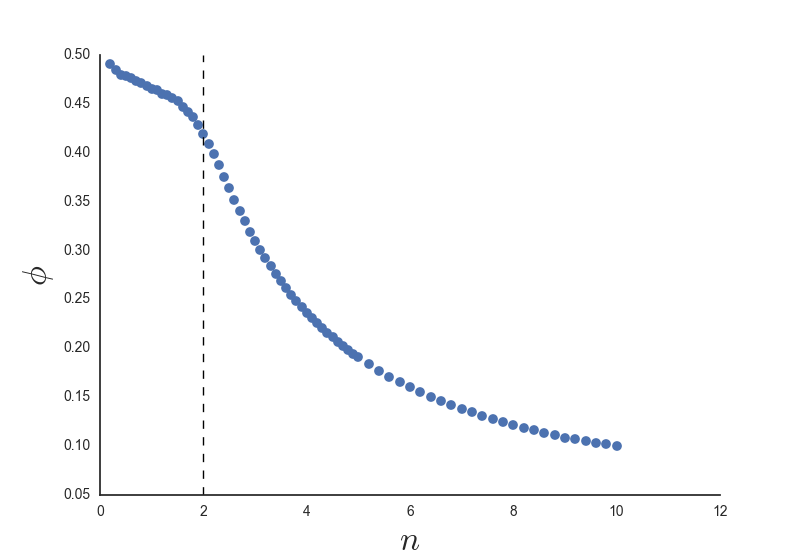
\includegraphics[width=0.65\textwidth]{figs_rle/s_pos.png}
  \caption{Fraction of active firms $\phi$ as a function of $n$, for $\epsilon = 0.005$ and $M=100$. At around $n=2$, the number of active firms collapses.}
  \label{fig:spos}
\end{figure}


To further characterize this transition, we show the results of numerical simulations for the fraction of active firms $\phi$ as a function of $n$, for $\epsilon = 0.01$ in Figure \ref{fig:spos}. We see that, indeed, there is a collapse in the fraction of active firms when $n = 2$, as predicted, when the number of active firms has reached its maximum and new firms either are immediately out of the market or replace old ones entirely, whereas when $n < 2$ new firms enter the market and with probability half operate among the incumbent ones. This effect can be seen even further on Figure \ref{fig:s_x_avg}, where we plot the average scale of production $\langle s \rangle$ for active firms, the spread reduction $\xi \cdot \delta x_0$ and $\langle x \rangle$ as a function of $n$. The interesting result is that when $n<2$, each new technology actually increases the average scale of production for all other firms, because it offers a new conversion possibility all firms can take advantage of. In the other hand, in the monopolistic regime, each new firm decreases the average scale of production because at the threshold, new firms only offer increasingly more specialized conversion rates that suit best the consumer's demand. However, the reduction in spread $\xi \cdot \delta x_0$ decreases roughly at the same rate, indicating that beyond $n=2$, new firms are simply replacing older, less efficient ones.

\begin{figure}[!ht]
  \centering
  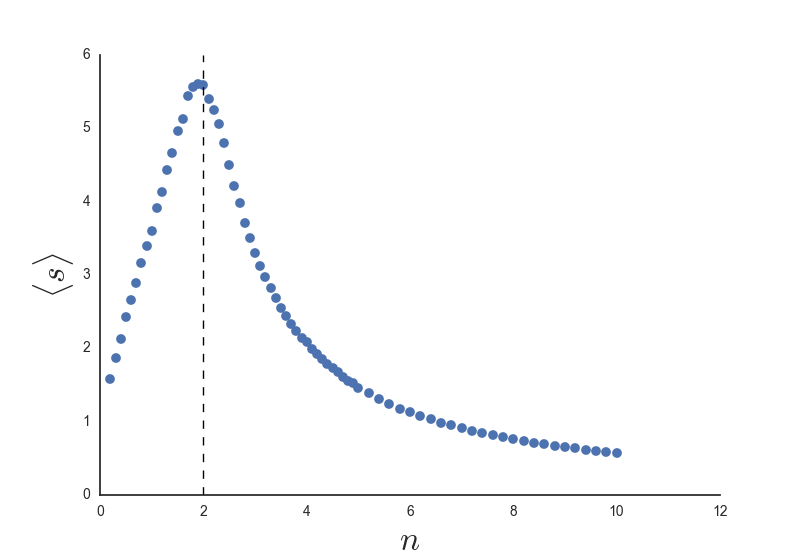
\includegraphics[width=0.32\textwidth]{figs_rle/s_avg.png}
  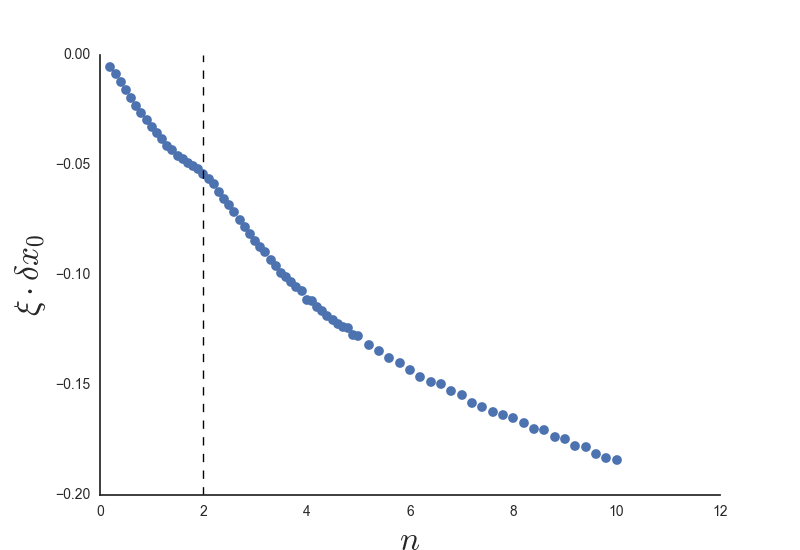
\includegraphics[width=0.32\textwidth]{figs_rle/spread_reduction.png}
  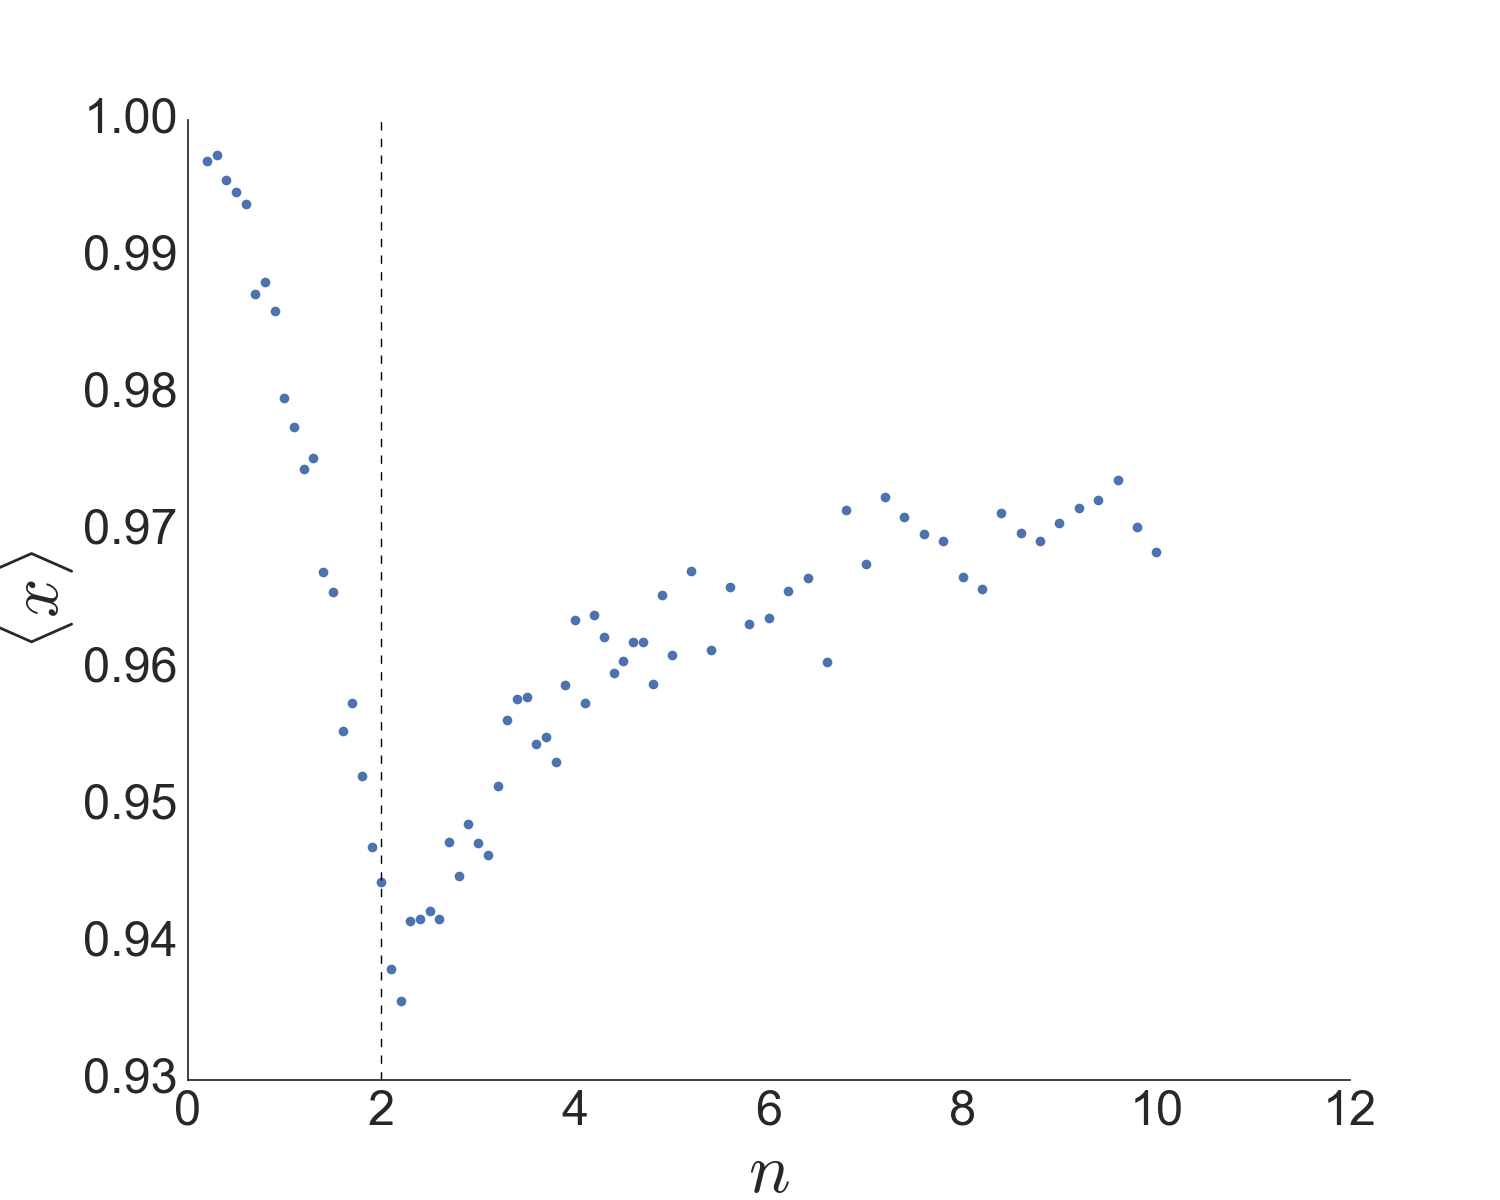
\includegraphics[width=0.32\textwidth]{figs_rle/x_avg.png}
  \caption{\textbf{(Left)} Average scale of production $s$ \textbf{(Middle)} Reduction in spread $\xi \cdot \delta x_0$ \textbf{(Right)} Average final bundle $\langle x \rangle$, all as a function of the technological density $n = \frac{N}{M}$. The plots show the regime change at $n=2$: when $n < 2$, in the competitive regime, each firm increases their production when a new technology enters the market, whereas the consumer is willing to sacrifice a bit more of his total amount of goods to increase his utility. At $n>2$, the monopolistic regime, the consumer doesn't sacrifice any more of his total amount of goods, and new firms are more efficient and decrease the average scale of all others. These results are from numerical simulations averaged over 1500 replicas, with $M=100$ and $\epsilon = 0.005$.}
  \label{fig:s_x_avg}
\end{figure}


The graph for $\langle x \rangle$ in Figure \ref{fig:s_x_avg} shows that the consumer too has a different behavior in the two regimes. In the competitive setting, firms are suboptimal and the consumer is able to maximize his utility only by sacrificing an increasingly larger amount of his initial endowment. Beyond $n=2$ the technologies are good enough that the consumer loses less when choosing an optimal bundle. In terms of utility, it increases rapidly with $n$ up until $n=2$ and it stalls a bit afterwards, showing the saturation of the economy, as shown in figure \ref{fig:u_GDP_avg}.

We can also define the gross product (GDP) for the
model as the total value of goods produced, that is, the sum of
$(x_\mu - x_0^\mu)p_\mu$ for all goods $\mu$ that are produced, i.e.,
$x_\mu > x_0^\mu$. Since market clearing condition
\eqref{eq:market_clearing_p} makes the value of goods produced equal
to the value of goods used as input, we calculate the GDP $Y$ by
averaging over the absolute value of all trades:

\begin{equation}
  \label{eq:GDP}
  Y = \frac{\sum_{\mu = 1}^M |x_\mu - x_0^\mu|p_\mu}{2 \sum_{\mu = 1}^M p_\mu},
\end{equation}
where the denominator also includes a normalization for the prices. The numerical results for the GDP are shown in figure \ref{fig:u_GDP_avg}, and, like the utility, it increases linearly with $n$ up until $n=2$, where it quickly stalls, another indicator that the economy enters a mature regime at this point. The utility and the GDP as a function of $n$ will be specially relevant in Chapter $\ref{cha:inefficient}$, when we will relax the zero temperature constraint.


\begin{figure}[!ht]
  \centering
  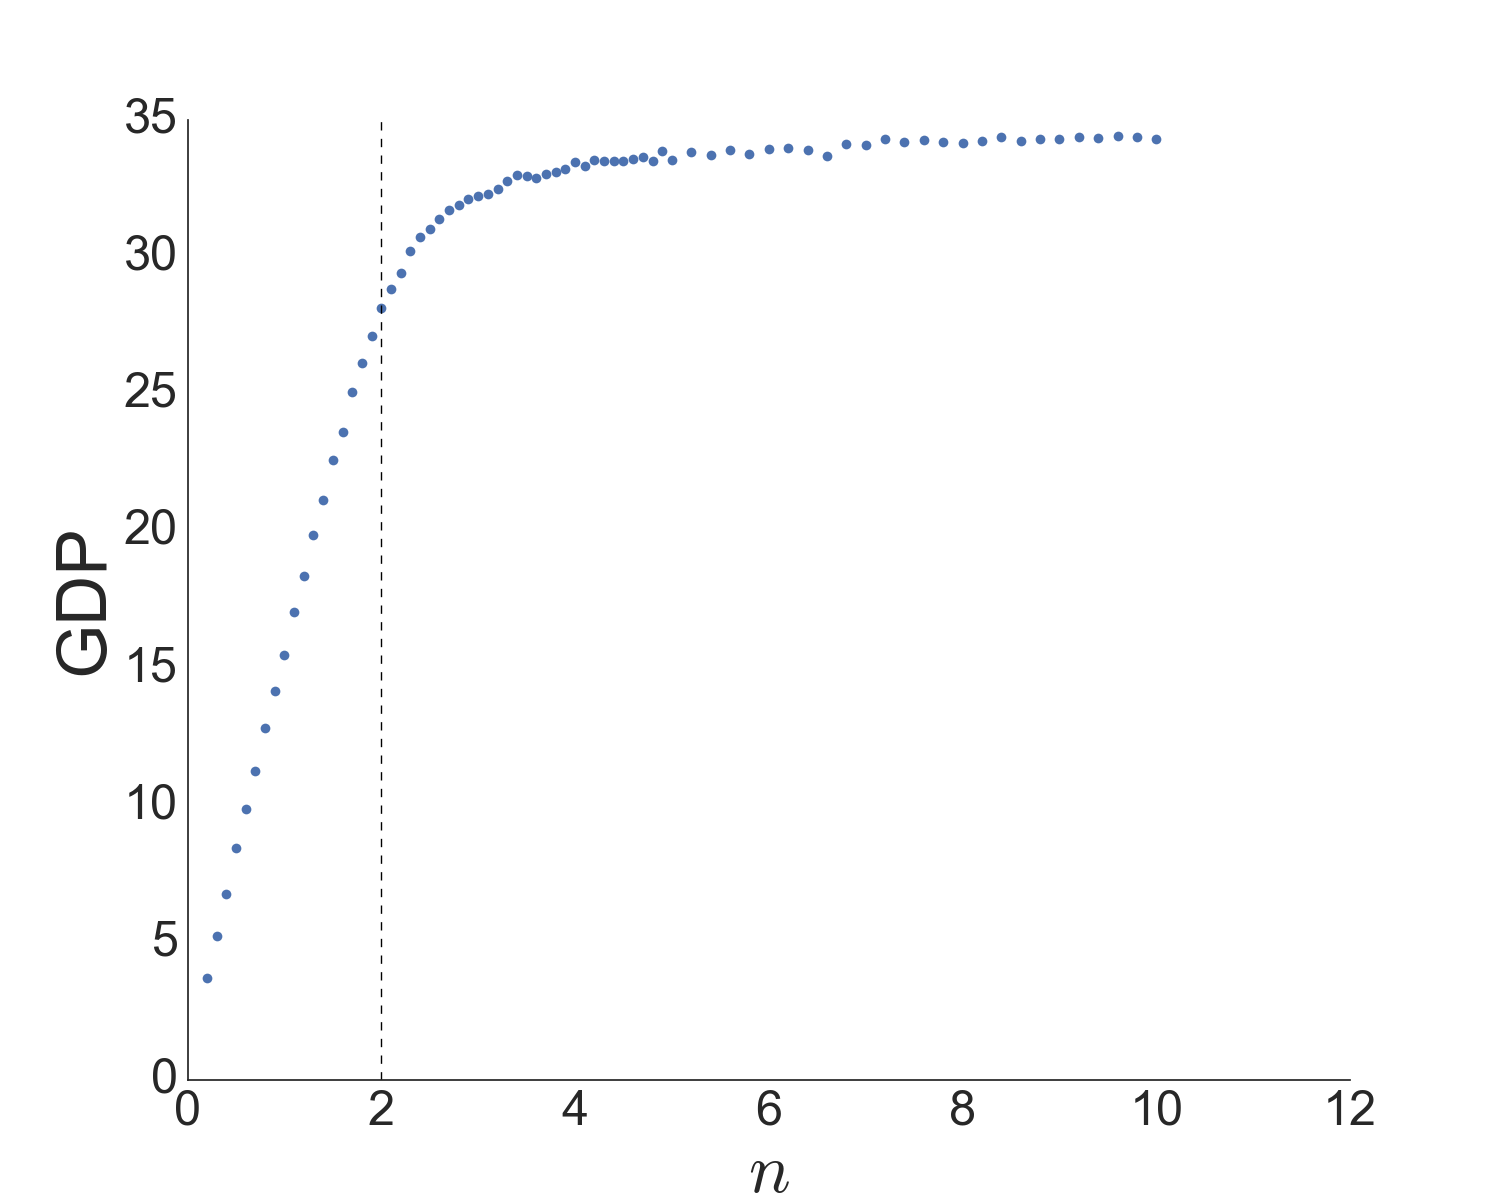
\includegraphics[width=0.45\textwidth]{figs_rle/gdp_avg.png}
  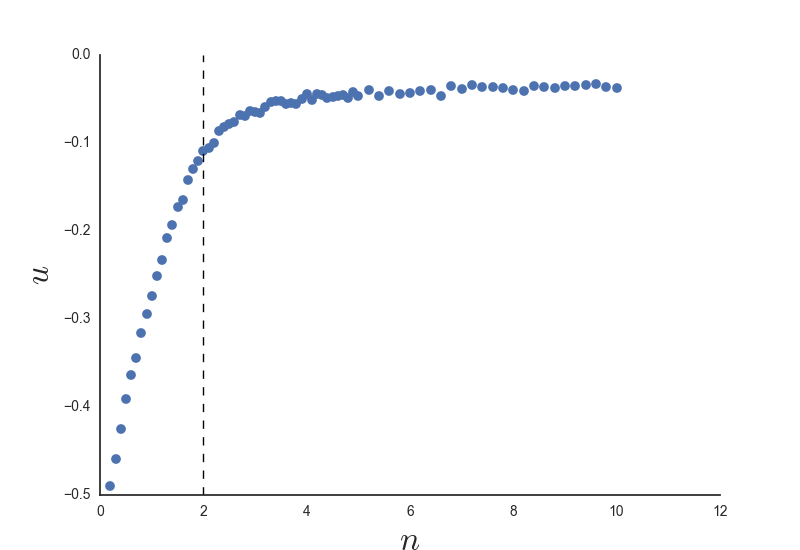
\includegraphics[width=0.45\textwidth]{figs_rle/utility_avg.png}
  \caption{\textbf{(Left)} Average GDP as defined by equation \eqref{eq:GDP} \textbf{(Right)} Average consumer utility per good, both as a function of the technological density $n$. Both increase rapidly as a function of new firms in the competitive regime $n < 2$ and saturate in the monopolistic regime $n >2$.}
  \label{fig:u_GDP_avg}
\end{figure}


The Random Linear Economies model is particularly suitable for further
analysis because it's a General Equilibrium setting with few
ingredients, but the introduction of stochastic elements offers a
nontrivial regime change which is not observed in similar
``simple'' economic models in the literature and are not solvable through standard economic maximization methods, as discussed in Chapter \ref{cha:stat_mech}.

For these reasons we used it as a basis for two of the applications presented in this thesis: in Chapter \ref{cha:inefficient} we will discuss how relaxing the $\beta \to \infty$ limit to arbitrary $\beta$ is a principled way of modeling an irrational consumer. On Chapter \ref{cha:IO} we will build Input-Output matrices for the model and compare to real world data.